\section{Experiments}
\label{sec:experiments}

This section describes our experiments and validates results.
We experimented with two different types of handles:
cuboids computed from PartNet~\cite{partnet} segmentations and
sphere-meshes computed from ShapeNet~\cite{shapenet} shapes using~\cite{spheremesh}.
We compare our results to two other approaches focused on generating shapes
as a set of simple primitives, namely cuboids~\cite{Tulsiani2017} 
and superquadrics~\cite{Paschalidou2019}.
All the experiments in the paper were implemented using Python 3.6
and PyTorch.
Computation was performed on TitanX GPUs.

\subsection{Datasets}
\paragraph{Cuboids from PartNet~\cite{partnet}.}
We experiment with human annotated handles by fitting cuboids to the parts
segmented in PartNet~\cite{partnet}.
The dataset contains 26,671 shapes from 24 categories and 573,585 part instances.
In order to compare our model with other approaches trained
on the ShapeNet~\cite{shapenet} chairs dataset, we select the subset of PartNet chairs
that is also present in ShapeNet.
This results in 6773 chair models segmented in multiple parts.
Every model has on average 18 parts, but there are also examples with as many as 137 parts.
For every part we fit a corresponding cuboid using PCA. 
Then, we compute the volume of every cuboid and keep at topmost 30 cuboids in terms of volume.
Notice that 92\% of the shapes have less than 30 cuboids, so those remain unchanged.
The others will have missing components, but those usually correspond to very small details
and can be ignored without degrading the overall structure.

\paragraph{Sphere-meshes from ShapeNet~\cite{shapenet}.}
In contrast to cuboids (which are computed from human annotated parts), we compute sphere-meshes fully automatically using the procedure
described in~\cite{spheremesh}.
%This means that we can apply this representation to any mesh repository and generate training data for our model.
We use ShapeNet categories that are also analyzed in~\cite{Paschalidou2019, Tulsiani2017}:
chairs, airplanes and animals.
The sphere-mesh computation procedure requires pre-selecting how many sphere-vertices to use.
The algorithm starts by considering the regular triangle mesh as a trivial sphere-mesh (vertices with null radius) and then decimates the
original mesh progressively through edge collapsing, optimizing for new sphere-vertex each time an edge is removed.
This procedure is iterated until the required number of vertices is achieved.

In our case, since our model is capable of generating sets with different cardinalities,
we are not required to set a fixed number of primitives for every shape. Therefore we use the following method to compute a sphere-mesh with adaptive number of vertices.
Specifically, for every shape in the dataset, we start by computing a sphere-mesh with
10 vertices. 
Then, we sample 10K points both on the sphere-mesh surface and the original mesh.
If the Hausdorff distance between the point clouds is smaller than $\epsilon=0.2$
(point clouds are normalized to fit the unit sphere), we keep the current computed sphere-mesh.
Otherwise, we compute a new sphere-mesh by incrementing the number of vertices.
This procedure continues until we reach a maximum of 40 vertices.
This adaptive sphere-mesh computation allows our model to achieve
a good balance between shape complexity and summarization --
simpler shapes will be naturally represented with a smaller number of primitives.
We note that the sphere-mesh computation allows the resulting mesh to contain not only triangles, but also edges (i.e. degenerate triangles).
For simplicity, we make no distinction between sphere-triangles or edges:
edges are simply triangles that have two identical vertices.


\begin{figure}[t]
\centering
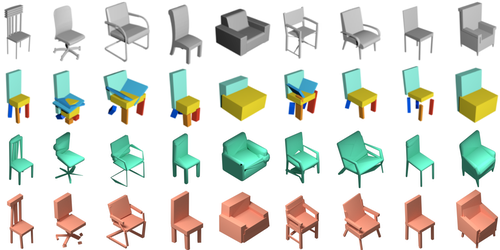
\includegraphics[width=1.0\linewidth]{handles/imgs/qualichairs.png}
\caption{\label{fig:chairs} \small
\textbf{Shape parsing on the chairs dataset}. From top to bottom, we show
ground-truth shapes,
results by Tulsiani et al.~\cite{Tulsiani2017}, results by our method using sphere-mesh handles, and our method using cuboids handles. 
Note how our results (last two rows) are able to generate handles with much better details such as the stripes on the back of the chair (first column),
legs on wheel chairs (second column) and armrests in several other columns.
}
\vspace{-10pt}
\end{figure}

\subsection{Shape Parsing}

The shape parsing task is to compute a small set of primitives from non-parsimonious,
raw, 3D representations, like occupancy grids, meshes or point clouds.
We analyze the ability of our model in performing shape parsing using a similar setup
to~\cite{Paschalidou2019, Tulsiani2017}.
Specifically, following the notation defined in Section~\ref{sec:method},
we train a model $f_\theta$ using input-output pairs $\langle x_i, S_i \rangle$, where
$x_i$ corresponds to a point cloud with 1024 points and $S_i$ is a set of handles
summarizing the shape represented by $x_i$.
We use a PointNet~\cite{pointnet} encoder to process
a point cloud with 1024 points and generate a 1024 dimensional encoding.
This encoding is then used as an input for our two-branched set decoder.
Both branches follow the same architecture: 3 fully connected layers with 256 hidden neurons
followed by batch normalization and ReLU activations.
The only difference between the two branches is in the last layer.
Assume $N$ is the maximum set cardinality generated by our model and $D$ is the handle
dimensionality (i.e. number of parameters of each handle descriptor, which happens to be $D=12$ for both sphere-mesh and cuboid). Then
$g_p$ outputs $N\times D$ values followed by a $\tanh$ activation, while $g_e$
outputs $N$ values followed by a sigmoid activation.
We set $N=30$ for cuboid handles and $N=50$ for sphere-meshes. %\duygu{in the previous section we said we used at most 40 vertices?} for sphere-meshes.
%\matheus{Yes, but the primitives are not vertices, but triangles. So the generated shapes can have at most 50 triangles, the training data can have more than that, but we just not consider the triangles with a smaller volume, just like the cuboids.}
The model is trained end-to-end by using the alternating training described in Section~\ref{sec:method}.
Training is performed using the Adam optimizer with a learning rate of $10^{-3}$ for 5K iterations
in each stage.

Figures~\ref{fig:chairs} and \ref{fig:all} show visual comparisons of our method with previous work. Qualitatively, our method generates shape handles with accurate geometric details, including many thin structures that previous methods struggle with. 

\begin{figure}
\centering
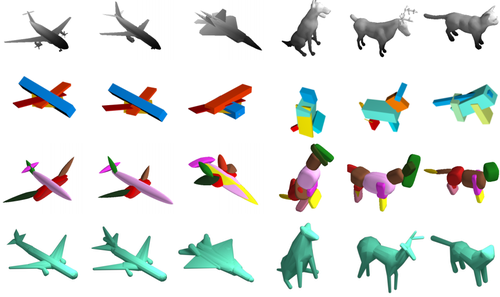
\includegraphics[width=1.0\linewidth]{handles/imgs/qualiall.png}
\vspace{-20pt}
\caption{\label{fig:all} \small
\textbf{Shape parsing on the airplanes and animals datasets}. From top to bottom, we show ground-truth shapes,
results by Tulsiani et al.~\cite{Tulsiani2017},
results by Paschalidou et al.~\cite{Paschalidou2019}, and results by our model trained using sphere-mesh handles.
Our results contain accurate geometric details, such as
the engines on the airplanes and animal legs that are clearly separated.
}
\end{figure}

\begin{table}[t]
\centering
\small
\begin{tabular}{l|l|ccc}
                   & \multirow{2}{*}{\textbf{Handle type}}  & \multicolumn{3}{c}{\textbf{Category}}        \\
                   &              & Chairs   & Airplanes & Animals \\
                   \hline
\cite{Tulsiani2017}    & Cuboid       & 0.129   & 0.065    & 0.334  \\
\cite{Paschalidou2019} & Superquadric & 0.141   & 0.181    & 0.751  \\
\hline
\multirow{ 2}{*}{Ours}               & Cuboid       & 0.311    & -         & -       \\
               & Sphere-mesh  & \textbf{0.298}    & \textbf{0.307}     & \textbf{0.761}      \\
\hline
%Oracle~\cite{spheremesh} & Sphere-mesh & 0.342 & & 0.768
\end{tabular}
\caption{
\label{tab:parse}
\textbf{Quantitative results for shape parsing.} Intersection over union computed
on the reconstructed shapes. The best self-supervised results are shown in bold font.
}
\end{table}

\paragraph{Quantitative comparisons}

We compare our method against~\cite{Tulsiani2017, Paschalidou2019} using intersection
over union (IoU) metric and results are shown in Table~\ref{tab:parse}.
As expected, when using cuboids as handles, our method leverages the annotated data from the PartNet~\cite{partnet} to achieve significantly more accurate shape
approximations (more than twice the IoU in comparison).
%Nevertheless, it is important to highlight that~\cite{Tulsiani2017, Paschalidou2019} are
%trained without utilizing man-made annotations.
On the other hand, as~\cite{Tulsiani2017, Paschalidou2019} are trained without leveraging annotated data, a more fair comparison is between theirs and our method using sphere-mesh handles, which are computed automatically.
Our method still clearly outperforms theirs in all categories --
chairs, airplanes and animals.
This shows that even though a neural network in theory should be able to learn the best parsimonious
shape representations, using self-supervision generated by shape summarization techniques (e.g. sphere-meshes) can still help it achieve more accurate approximations. 
%e.g., 0.298 vs. 0.141 for chairs, 0.307 vs. 0.181 for airplanes, when compared
%with~\cite{Paschalidou2019} in terms of intersection over union.
%Furthermore, our method is capable of leveraging man-made shape handles to get even
%better shape approximations -- an improvement from 0.298 to 0.311 when generating
%chairs using cuboids from PartNet instead of automatically computed sphere-meshes. 
%\rui{this last point is a bit tricky: one can argue while cuboid leverages annotated data, it's also a less accurate type of handle, so it's not immediately clear why it should win.}
%As a side note, it is important to discuss the results for the animals category.
%We noticed that this dataset is quite small (only 129 shapes) and shapes from test and training splits
%are very similar.
%Thus, a method capable of overfitting to the training set will likely get a very good approximation.
%This explains why all the methods perform better in this dataset and why
%the performance of our method is very close to the sphere-mesh computation done through~\cite{spheremesh}, which provides supervision for our approach.

\begin{figure}[t]
\centering
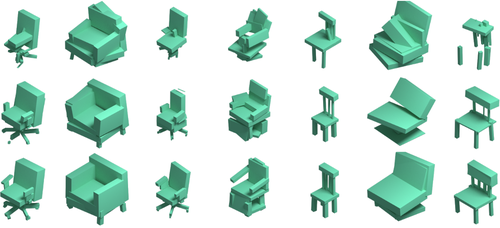
\includegraphics[width=1.0\linewidth]{handles/imgs/ablation.png}
\vspace{-15pt}
\caption{\label{fig:abl} \small
\textbf{Ablation studies.}
Shapes generated from a model trained without our proposed handle similarity metric (first row),
model trained without the two-stage training procedure (second row), and our full model (last row).
Note that comparing handles using just $\ell_2$-norm (first row) yields poor results.
Training $g_p$ and $g_e$ at the same time (instead of alternating) yields reasonable results, but some parts
are missing and/or poorly oriented.
}
\end{figure}
\begin{table}[]
\centering
\begin{tabular}{ccc}
\hline
w/o similarity & w/o alternate & full model \\
0.192 & 0.320 & \textbf{0.352}\\
\hline
\end{tabular}
\caption{ \small
\label{tab:abl}
Quantitative results of ablation studies comparing our full model with two variations that lack our handle similarity metric and alternate training procedure respectively.
}
\vspace{-0.1in}
\end{table}

\subsection{Ablation studies}
\label{sec:ablation}
We investigated the influence of the two main contributions of this work:
the similarity metric for handles and the alternating training procedure for $g_p$ and $g_e$.
To do so, we adopt a shape-handle auto-encoder and compare different variations by computing
the IoU of reconstructed shapes in a held-out test set.
The auto-encoder architecture is very similar to the one used in shape parsing, except for
the encoder -- it still follows a PointNet architecture, but every ``point'' is actually
a handle treated as a point in a $D$-dimensional space.
We analyzed three different variations.
In the first one, we simply used the $\ell_2$-norm between the handle parameters (cuboids, in this case).
As shown in Figure~\ref{fig:abl} and Table~\ref{tab:abl},
the proposed handle similarity metric has a significant impact on the quality of the
generated shapes.
The second variation consists of training the same model, but without using the alternating procedure
described in Section~\ref{sec:method}. %, where first $g_p$ is trained by only minimizing $C(z,S)$ and later $g_e$ is trained minimizing the full loss $\mathcal{L}_{rec}$. 
Figure~\ref{fig:abl} shows that the alternating training procedure generates
more accurate shapes, with fewer missing parts and better cuboid orientation.


\subsection{Applications}
\label{sec:applications}
In this section, we demonstrate the use of our generative model in several applications.
We employed a Variational Auto-Encoder (VAE)~\cite{vae} for this purpose.
It follows the same architecture as the auto-encoder described in Section~\ref{sec:ablation} with the 
only difference being that the output of the encoder (latent representation $z$) has
dimensionality 256 instead of 512.
Additionally, following~\cite{mrt18}, we added an additional regularization term to the training objective:
\begin{equation}
    \mathcal{L}_{reg} = \norm{cov(Q(x) + \delta)}_2 + \mathbb{E}_{x\sim\mathcal{D}}[Q(x)]
\end{equation}
where $Q$ is the encoder, $cov(\cdot)$ is the covariance matrix, $\norm{\cdot}_2$ is the Frobenius norm, $x$ is input handle set and $\delta$ is random noise sampled from $\mathcal{N}(0,cI)$.
Thus, the network is trained minimizing the following function:
\begin{equation}
    \mathcal{L} = \mathcal{L}_{rec} + \lambda\mathcal{L}_{reg}.
\end{equation}
In all our experiments, we used $\lambda=0.1$ and $c=0.01$.
The model is trained using the alternate procedure described before, \ie $\mathcal{L}_{rec}$ is replaced by $C(z,S)$ while training $g_p$.

\vspace{5pt}
\noindent\textbf{Interpolation.}
\begin{figure}
\centering
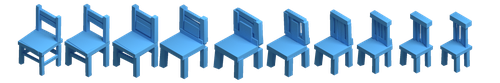
\includegraphics[width=1.0\linewidth]{handles/imgs/interpolation.png}
\vspace{-20pt}
\caption{\label{fig:interp} \small
\textbf{Latent space interpolation}
Sets of handles can be interpolated by linearly interpolating
the latent representation $z$.
Transitions are smooth and generate plausible intermediate shapes.
Notice that the interpolation not only changes handle parameters, but also
adds new handles / removes existing handles as necessary.
}
\vspace{-15pt}
\end{figure}
Once the VAE model is trained, we are able to morph between two shapes by 
linearly interpolating their latent representations $z$.
In particular, we sample two values $z_1, z_2$ from $\mathcal{N}(0, I)$ and generate new shapes by passing the interpolated encodings $\alpha z_1 + (1-\alpha) z_2$ through the decoder $g$,
where $\alpha \in [0, 1]$.
Results using cuboid handles are presented in Figure~\ref{fig:interp}.
Note that the shapes are smoothly interpolated, with new handles added and old handles removed as necessary when the overall shape deforms.
Additionally, relationships between handles, 3.4.4.0.1    Shape editing.like symmetries, adjacency and support, are
preserved, thanks to the latent space learned by our model, even though such characteristics are never explicitly specified as supervision.

\vspace{5pt}
\noindent\textbf{Handle completion.}
Consider an incomplete set of handles $A=\{a_i\}_{i=1}^{N}$ as input, the handle completion task is to generate a complete set of handles $A^*$,
such that $A^*$ contains not only the handles in the input $A$ but also necessary additional handles that result in a plausible shape.
For example, given a single cuboid handle as shown in Figure~\ref{fig:completion},
we want to generate a complete chair that contains that input handle.
We perform this task by finding a latent representation $z^*$ that generates a set of handles approximating the elements
in $A$. Specifically, we solve the following optimization problem:
\begin{equation}
   z^* = \argmin_{z \in \mathcal{Z}}C(z, A), \quad A^* = g(z^*),
   \label{eq:completion}
   \vspace{-5pt}
\end{equation}
where $C$ is the coverage metric defined in Equation~\ref{eq:cov} and $A^*$ is the completed shape (i.e. output of the decoder using $z^*$ as input).
We can also use the existence prediction branch ($g_e$) in this framework to reason
about how complex we want the completed shapes to be.
Specifically, we add an additional term to the optimization:
\begin{equation}
    \label{eq:completion}
   z^* = \argmin_{z \in \mathcal{Z}}C(z, A) + \gamma\sum_{i=1}^{N}[g_e(z)]_i,
   \vspace{-5pt}
\end{equation}
where $\gamma$ controls the complexity of the shape.
If $\gamma=0$, we are not penalizing a set with multiple handles -- only
coverage matters.
As $\gamma$ increases, existence of multiple handles is penalized more, leading to a solution with a lower cardinality.
As can be seen in Figure~\ref{fig:completion}, our model is capable of recovering plausible chairs even when given a single handle. In addition, we can generate multiple proposals for $A^*$ by initializing the optimization with different values of $z$. More results can be found in the supplemental material. 
%Finally, that figure also shows how we can control the complexity of the output shape by varying the value of $\gamma$. 
%Additionally, 

\begin{figure}
\centering
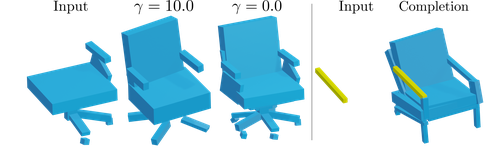
\includegraphics[width=1.0\linewidth]{handles/imgs/completion.png}
\vspace{-18pt}
\caption{\label{fig:completion} \small
\textbf{Results of handle completion}.
Recovering full shape from incomplete set of handles.
Using $\gamma$ to control the complexity of the completed shape (left).
Predicting a complete chair from a single handle (right).
}
\vspace{-0.1in}
\end{figure}

%\vspace{5pt}\noindent\textbf{Shape editing.}
\paragraph*{Shape editing.}
For editing shapes, we use a similar optimization based framework.
Consider an original set of handles $A$ describing a particular shape.
Assume that the user made edits to $A$ by modifying the parameters of some handles, creating
a new set $A^\prime$.
Our goal is to generate a plausible new shape $A^*$ from $A^\prime$, while minimizing the deviation 
from the original shape.
To achieve this goal, we solve the following minimization problem via gradient descent:
\begin{equation}
   \label{eq:Editing}
   z^* = \argmin_{z \in \mathcal{Z}}C(z, A^\prime) + \gamma\norm{z - z_A}_2, \quad A^* = g(z^*)
\end{equation}
where $z_A$ is the latent representation of the original shape.
The intuition for Equation~\ref{eq:Editing} is simple: we want to generate a plausible shape that
approximates the user edits by minimizing  $C(z, A^\prime)$ but also keep the overall
characteristics of the original shape $A$ by adding a penalty for deviating
too much from $z_A$.
Results are shown in Figure~\ref{fig:editing}. 
As observed in the figure, when the user edits one of the handles, 
our model can automatically modify the shape of the entire chair while preserving its overall structure. 

\begin{figure}3.4.4.0.1    Shape editing.
\centering
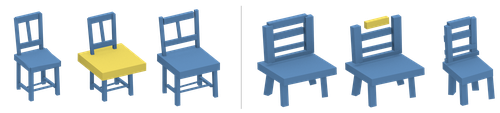
\includegraphics[width=1.0\linewidth]{handles/imgs/editing.png}
\vspace{-20pt}
\caption{\label{fig:editing} \small
\textbf{Editing chairs}.
Given an initial set of handles, a user can modify any handle (yellow). Our model then
updates the entire set of handles, resulting in a modified shape which observes the user edits while preserving the overall structure.}
\vspace{-0.2in}
\end{figure}

%\vspace{5pt}
%\noindent\textbf{Limitations.}
\paragraph*{Limitations.}
Our method has several limitations to be addressed in future work. 
First, during training we set a maximum number of handles to be generated. 
Increasing this number would allow more complex shapes but also entail a larger network with higher capacity. 
Therefore, there is a trade-off between the compactness of the generative model and the desired output complexity. 
Furthermore, our method currently does not guarantee the output handles observe certain geometric constraints, such as parts that need to be axis-aligned or orthogonal to each other. 
For man-made shapes, these are often desirable constraints and even slight deviation is immediately noticeable. 
While our model can already learn geometric relationships among handles from the data directly, generated shapes might benefit from additional supervision enforcing geometric constraints. 

%GRASS~\cite{li_sig17} and StructureNet~\cite{mo2019structurenet}
%Furthermore, we are modeling the shapes as sets of handles.
%Also, adding more handles might not be desirable, since we want to keep the shape representations easy to manipulate.
%Finally, in contrast to , which model shapes as graphs, our model
%does not explicitly generate relationship between parts (symmetry, support, etc).
%On the other hand, our model does not require this extra annotation and it is capable
%of learning some of these relationships directly from data.
